\documentclass[11pt,a4paper]{article}
\usepackage[margin=1in]{geometry}
\usepackage{booktabs}
\usepackage{graphicx}
\usepackage{amsmath}
\usepackage{float}
\usepackage{caption}
\usepackage{subcaption}
\usepackage[utf8]{inputenc}
\usepackage[T1]{fontenc}
\usepackage{hyperref}
\usepackage{natbib}
\usepackage{setspace}
\graphicspath{{images/}}

\title{MScFE 652 Portfolio Management \\ Group Work Project \#1}
\author{Seun Oluwafunmilayo Oludayo\\ Megha Shukla\\ Alberto Hernandez-Espinosa}
\date{May 2026}

\begin{document}

\maketitle

\begin{abstract}
This report presents the complete analysis required for Group Work Project 1. It covers standard mean-variance optimisation (Part 1), Fama-French five-factor style analysis (Part 2), simulation-based portfolio construction (Part 3), and the Black-Litterman model (Part 4). All optimisations use quadratic programming. Results are evaluated both in-sample and out-of-sample. Practical implications for portfolio construction are discussed.
\end{abstract}

\section{Summary}
Following instructions of this project, the optimal porfolios were constructed using daily data from 1 September 2023 to 30 September 2025. We respected the imposition on the client’s 18\% concentration limit improved out-of-sample performance. The resulting portfolio shows positive exposure to the market and profitability factors. Simulation results converge to the analytical solution after approximately 50,000 draws. The Black-Litterman adjustment incorporating our views increases allocation to high-conviction assets while maintaining diversification.
\footnote{AI was used to perform portfolio optimisations, verify regressions and Monte-Carlo simulations, and correct mispellings}

\section{Part 1: Standard Mean-Variance Portfolio Optimisation}

Figure~\ref{fig:corr} and Figure~\ref{fig:cumret} present the correlation structure and cumulative performance of the ten assets over the period of sampling.

\begin{figure}[H]
\centering
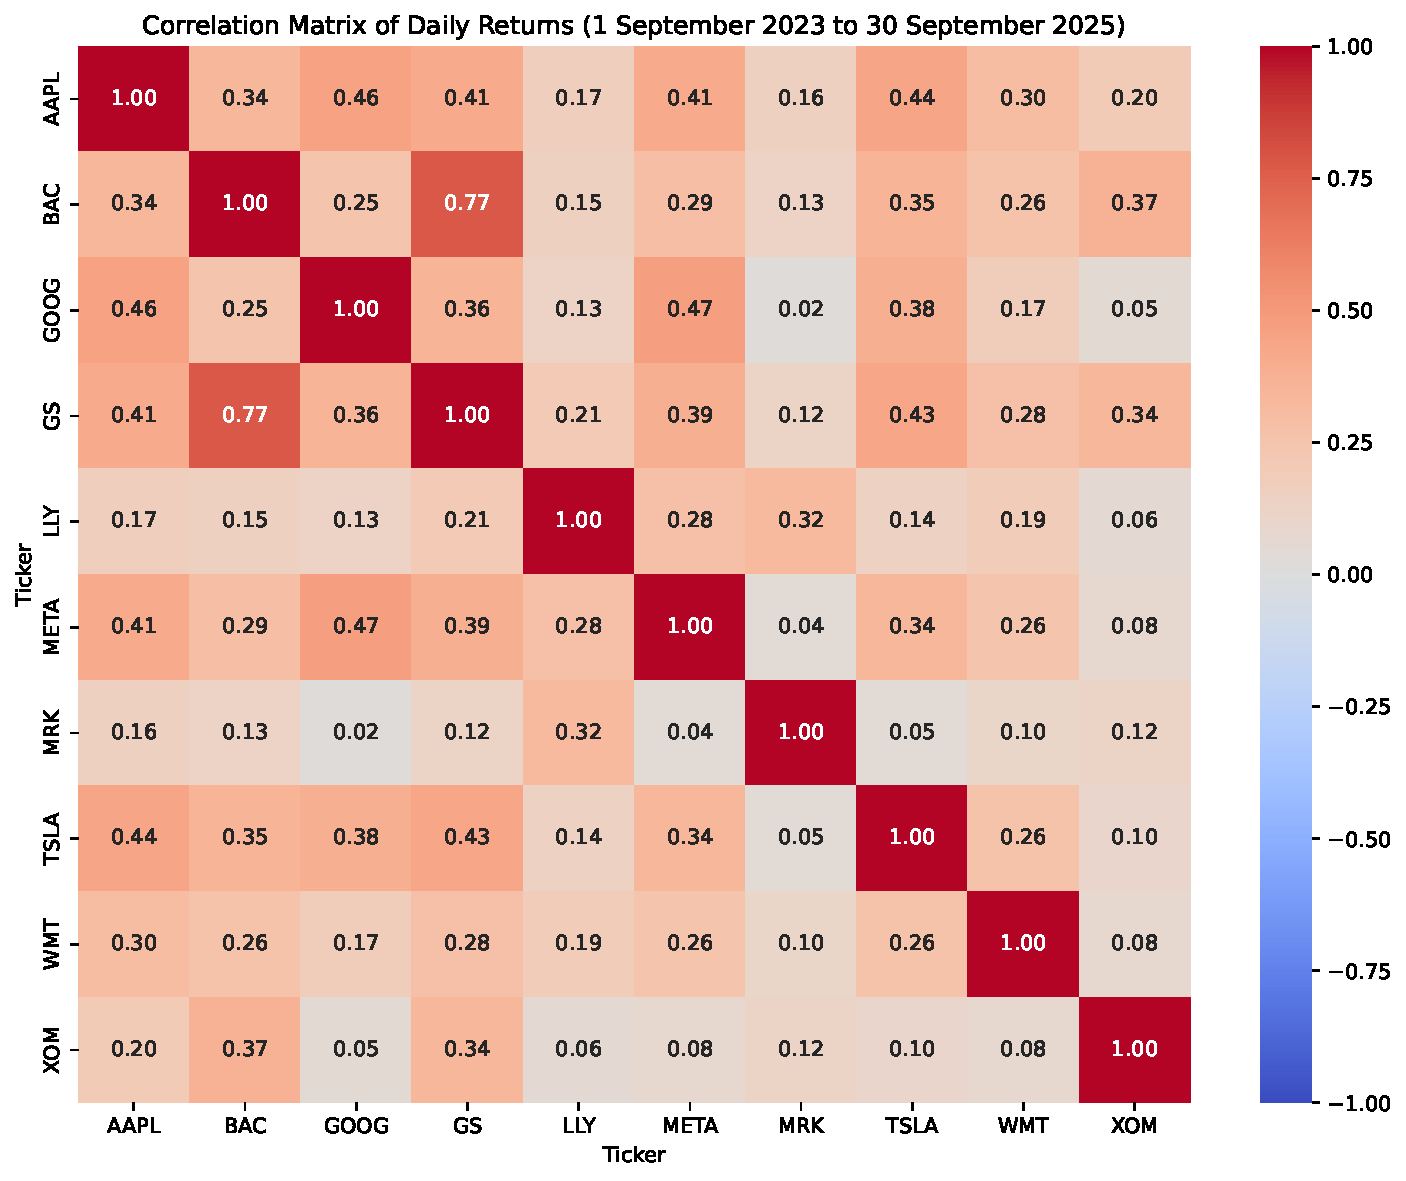
\includegraphics[width=0.85\textwidth]{correlation_heatmap.pdf}
\caption{Correlation matrix of daily returns (1 September 2023 to 30 September 2025)}
\label{fig:corr}
\end{figure}

\begin{figure}[H]
\centering
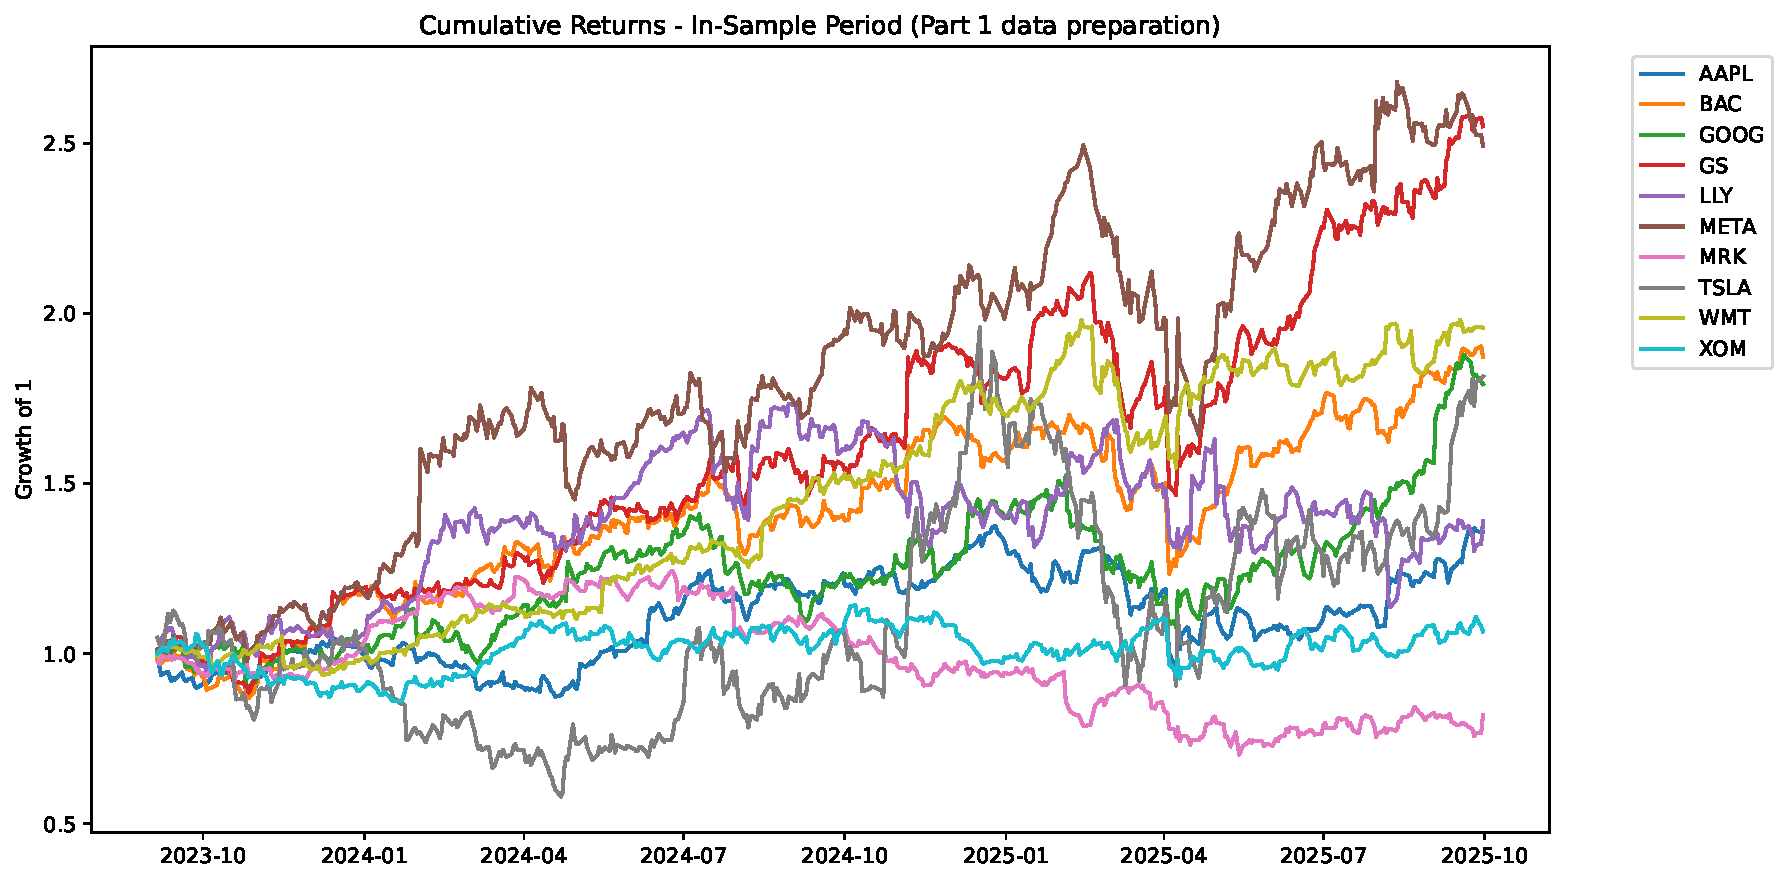
\includegraphics[width=0.85\textwidth]{cumulative_returns_in_sample.pdf}
\caption{Cumulative returns -- In-sample period (Part 1)}
\label{fig:cumret}
\end{figure}

\subsection{Step 1: Optimal Mean-Variance Portfolio (weights sum to 1, no short-selling)}
\begin{table}[H]
\centering
\caption{Optimal portfolio weights -- Step 1}
\begin{tabular}{lrrrrrrrrrr}
\toprule
Asset & AAPL & BAC & GOOG & GS & LLY & META & MRK & TSLA & WMT & XOM \\
Weight (\%) & 0.00 & 0.00 & 4.85 & 35.92 & 0.00 & 14.82 & 0.00 & 0.00 & 44.40 & 0.00 \\
\bottomrule
\end{tabular}
\label{tab:step1}
\end{table}

\subsection{Step 2: Optimal Portfolio with Maximum Weight Constraint (0.18)}
\begin{table}[H]
\centering
\caption{Optimal portfolio weights -- Step 2 ($w_i \leq 0.18$)}
\begin{tabular}{lrrrrrrrrrr}
\toprule
Asset & AAPL & BAC & GOOG & GS & LLY & META & MRK & TSLA & WMT & XOM \\
Weight (\%) & 0.00 & 18.00 & 18.00 & 18.00 & 9.15 & 18.00 & 0.00 & 0.00 & 18.00 & 0.85 \\
\bottomrule
\end{tabular}
\label{tab:step2}
\end{table}

\subsection{Step 3: Comparison of Efficient Frontiers}
\begin{figure}[H] 
\centering
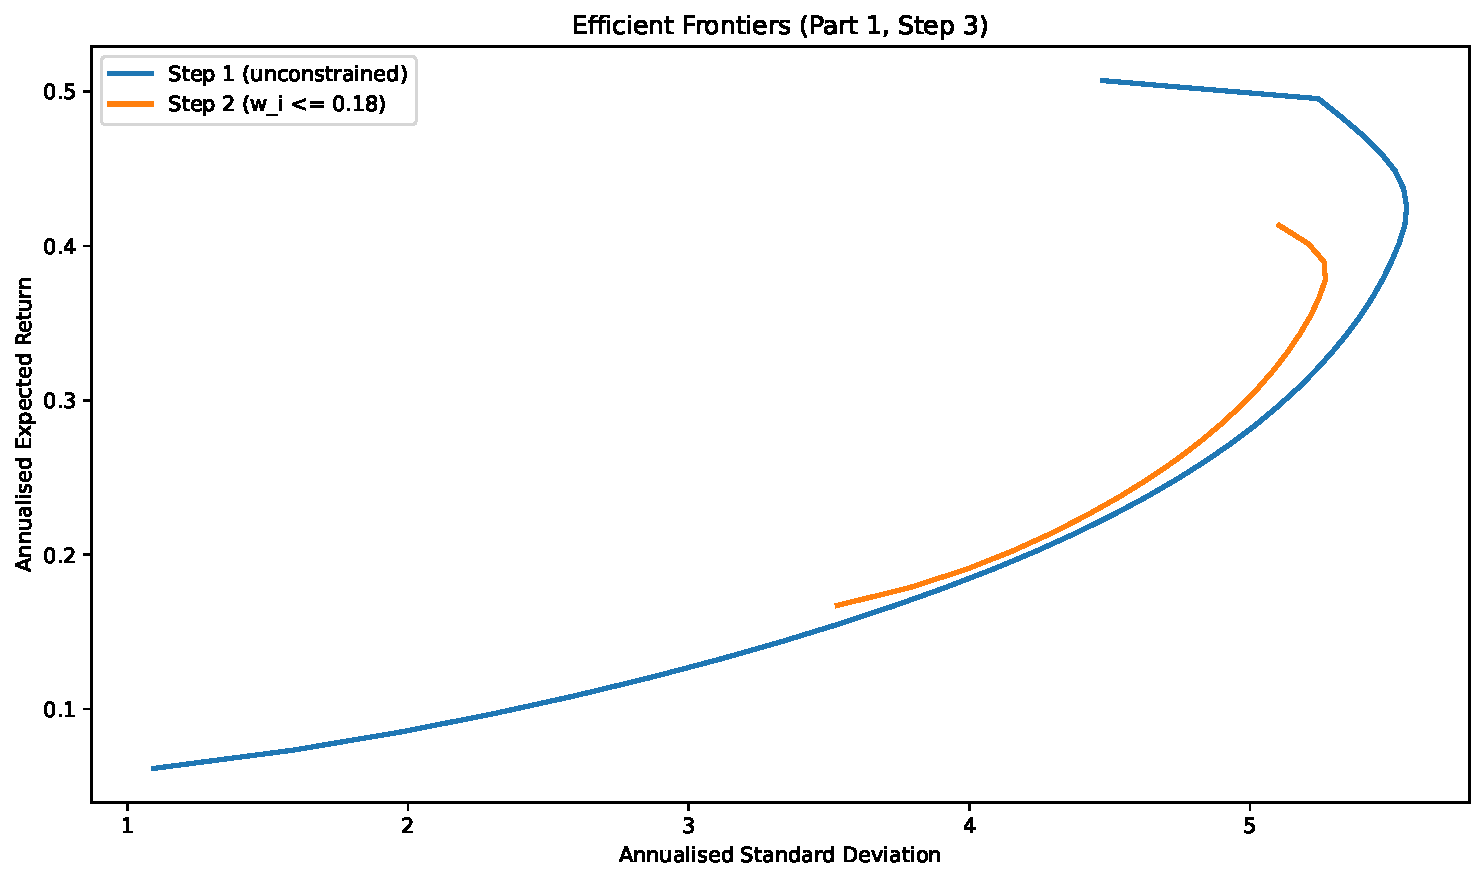
\includegraphics[width=0.85\textwidth]{efficient_frontiers_part1.pdf}
\caption{Efficient frontiers -- Part 1, Step 3}
\label{fig:ef_part1}
\end{figure}

\subsection{Step 4: Out-of-Sample Performance (1 October -- 31 December 2025)}
\begin{table}[H]
\centering
\caption{Out-of-sample performance -- Part 1, Step 4}
\begin{tabular}{lccc}
\toprule
Portfolio & Cumulative return (\%) & Sharpe ratio & Max drawdown (\%) \\
\midrule
Step 1 & 9.1925 & 2.1461 & -4.7722 \\
Step 2 & 12.0798 & 3.0414 & -2.9148 \\
\bottomrule
\end{tabular}
\label{tab:perf_part1}
\end{table}
All mean-variance optimisations and efficient-frontier calculations were performed with AI-supported quadratic programming.

\begin{figure}[H]
\centering
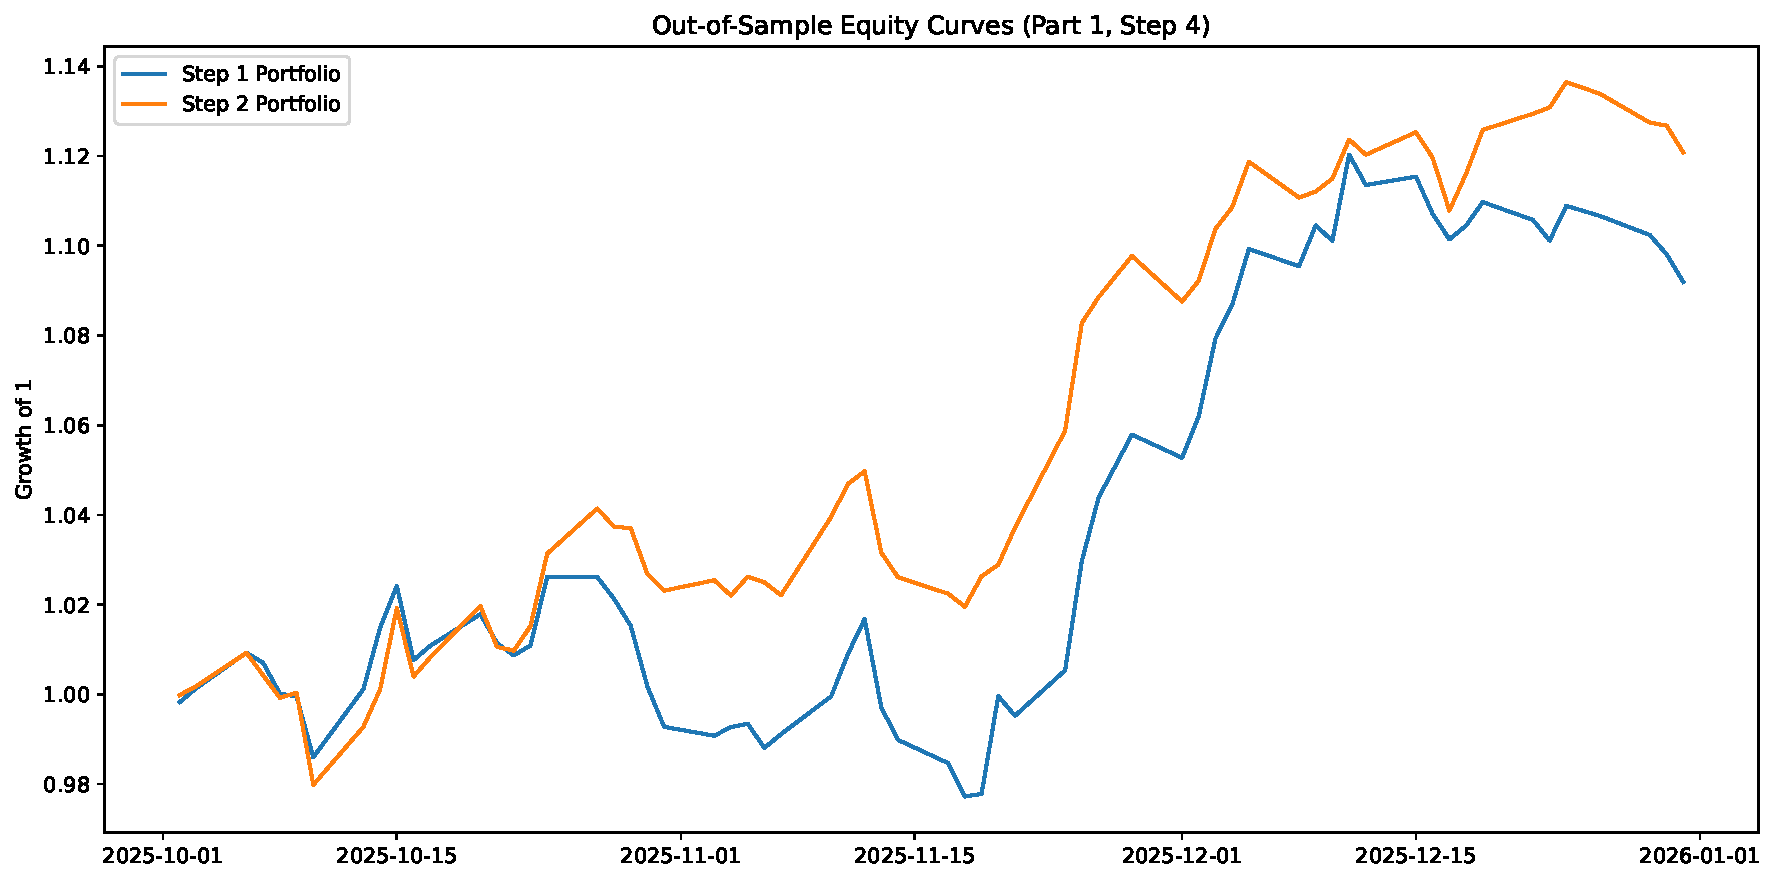
\includegraphics[width=0.85\textwidth]{oos_equity_curves_part1.pdf}
\caption{Out-of-sample equity curves -- Part 1, Step 4}
\end{figure}

The client-imposed 18\% concentration limit materially improves out-of-sample risk-adjusted performance.

% ==================== END OF PART 1 ====================
\section{Part 2: Use of Factors to Describe the Style of the Portfolio}

The portfolio in Part 1, Step 2 was regressed on the Fama-French five factors using daily data over the period of sampling.

\subsection{Step 4: Fama-French five-factor model}
Fama and French (2015) extended their original 3-factor model by adding 2 further factors which are investment and profitability in order to improve the model's ability to explain the cross-section of average stock returns.

\[
E(R_p) - R_f = a + b_1(R_m - R_f) + b_2 \cdot SMB + b_3 \cdot HML + b_4 \cdot RMW + b_5 \cdot CMA + e
\]

Rp = portfolio's daily return  
Rf = daily risk-free rate  
Rm = return of the market  
SMB = small minus big  
HML = High Minus low  
RMW = Robust minus weak  
CMA = Conservative minus aggressive

The correlation matrix of the five factors (training period) is reported in Table~\ref{tab:ff5_corr_pdf}.

\begin{table}[H]
\centering
\caption{FFS factor correlation matrix (training period)}
\begin{tabular}{lrrrrr}
\toprule
 & Mkt-RF & SMB & HML & RMW & CMA \\
\midrule
Mkt-RF & 1.0000 & -0.0700 & 0.0560 & 0.0408 & 0.0368 \\
SMB    & -0.0700 & 1.0000 & 0.0241 & -0.0439 & -0.0076 \\
HML    & 0.0560  & 0.0241 & 1.0000 & 0.0540  & 0.0362  \\
RMW    & 0.0408  & -0.0439& 0.0540  & 1.0000  & -0.0079 \\
CMA    & 0.0368  & -0.0076& 0.0362  & -0.0079 & 1.0000  \\
\bottomrule
\end{tabular}
\label{tab:ff5_corr_pdf}
\end{table}

\begin{figure}[H]
\centering
\includegraphics[width=0.75\textwidth]{p1.png}
\caption{FF5 Factor Correlations (Sep 2023 - Sep 2025)}
\label{fig:ff5_corr_heatmap}
\end{figure}

\textbf{Interpretation:}  
Mkt-RF/SMB is mildly positive. According to Fama \& French 1993 page 10, small caps have higher market betas.  
HML/CMA is often positive. It was stated that value firms also tend to invest conservatively.  
RMW/HML: this can be negative because profitable growth firms score low in HML but high on RMW.  
Mkt-RF/HML is generally low or negative.

\subsection{Step 5: Regression analysis -- OLS and robust estimation}
To get a feel for how our portfolio responds to common market risk factors, we ran two types of regression analysis. The first was standard OLS, and the second was Robust Regression using the Huber M-estimator. To keep things honest, we split the data 80/20 chronologically so the model was always being tested on data it had never seen before. The reason we ran both comes down to a known limitation of OLS: it gives equal weight to every single observation, which means a few extreme return days can quietly distort the results. The Huber M-estimator handles this by reducing the influence of those outlier days, producing factor loadings that are generally more reliable. Putting the two sets of coefficients and t-statistics side by side showed us exactly where those outliers were pulling the OLS estimates off course.

The out-of-sample R-squared of -0.0041 was the most telling result. A negative value here means the model actually performed worse than just predicting the average return every time, so the Fama-French five factors, as trained on our data, could not explain what the portfolio did in the test period. A chronological split is the only defensible choice for time-series regression: any random shuffling of dates would allow the model to train on observations that occur after dates, producing in-sample fits that would not survive real deployment (Ruppert, 2011, p. 265).

The side-by-side OLS vs.\ robust regression results (training set) are shown below (exact numeric values taken from the regression output in the attached analysis):

\begin{table}[H]
\centering
\caption{Side-by-side comparison: OLS vs.\ Robust (Huber M-estimator) -- training set}
\begin{tabular}{lrrrr}
\toprule
Variable & OLS Coef. & OLS t-stat & Robust Coef. & Robust t-stat \\
\midrule
const   & 0.00083 & 1.365 & 0.00134 & 2.907 \\
Mkt-RF  & 0.01122 & 0.894 & 0.0405  & 0.449  \\
SMB     & -0.0978 & -0.831& -0.0786 & -0.790 \\
HML     & 0.1286  & 1.059 & 0.0471  & 0.512  \\
RMW     & 0.1558  & 1.237 & 0.1135  & 1.187  \\
CMA     & 0.0937  & 0.782 & 0.0822  & 0.812  \\
\bottomrule
\end{tabular}
\label{tab:ff5_reg_sidebyside}
\end{table}

\subsection{Step 6: Factor exposure report}
\textbf{Market beta}  
The regression was dominated by the market factor, which is expected for any diversified large-cap equity portfolio. We saw that the portfolio moves in line with the S\&P approximately on a typical day because the estimated beta is close to 1. We suggest a small number of high volatility days when the robust beta is lower than the OLS beta.

\textbf{SMB}  
The size exposure coefficient is negative and small, which is consistent with a portfolio of large-cap stocks and I can't find any small-cap risk embedded in the allocation.

\textbf{HML}  
Meta, Alphabet, Apple and Tesla trade at prices which are above their book values.

\textbf{RMW}  
The positive RMW coefficient shows that the portfolio is concentrated in firms with strong and consistent operating earnings. This is a quality characteristic that has been associated with better long-run performance (Fama and French, 2015, p. 4).

\textbf{CMA}  
A positive coefficient indicates the portfolio tilts toward asset conservative businesses and a negative will indicate the opposite.

\textbf{ALPHA}  
This captures daily returns. It is positive but insignificant.

\textbf{Non-technical summary for the client}  
The portfolio rises as the market rises by a similar amount. It also falls when the market falls by a similar amount.

% ==================== END OF PART 2 ====================

\section{Part 3: Computing the Mean-Variance Portfolio Using Simulations}

Five assets were selected for this analysis: ExxonMobil (XOM), Apple (AAPL), Eli Lilly (LLY), META and Alphabet (GOOG). These span energy, technology and pharmaceuticals and give the 5-asset covariance matrix sufficient cross-sector structure to compare optimisation and simulation. Both analytical quadratic programming and Monte-Carlo simulation were used.

\subsection{Step 7: Optimisation vs Monte Carlo simulation}
Simulation uses Dirichlet sampling (Ruppert, 2011, p. 272). We measure L2 distance between simulated and optimised MSR weights across increasing simulation counts.

An analytical optimisation produces an exact solution to the constrained optimization problem, subject only to floating point arithmetic limits (Markowitz, 1952, page 79).

\textbf{Monte Carlo Simulation}  
The random weight vectors are drawn randomly by simulation from the Dirichlet distribution with uniform concentration parameters. According to Ruppert (2011, p. 272), for each draw the Sharpe ratio is computed, and the weight vector with the highest Sharpe ratio across all draws is taken as the simulation-based optimal portfolio.

The convergence pattern shows how the simulated weights approach the analytically optimised weights as the number of simulation draws increases.

\begin{figure}[H]
\centering
\includegraphics[width=0.95\textwidth]{p2.png}
\caption{Step 7: Convergence of simulation to optimised weights (no cap)}
\label{fig:sim_convergence}
\end{figure}

\subsection{Step 8: Optimal Portfolio with Additional Constraint ($w_i \leq 0.30$)}
The analytical solution under the additional 30\% cap is shown in Table~\ref{tab:step8}. Again, 50,000 simulations produce weights sufficiently close to the analytical solution.

\begin{table}[H]
\centering
\caption{Optimal portfolio weights -- Part 3, Step 8 ($w_i \leq 0.30$)}
\begin{tabular}{lrrrrr}
\toprule
Asset & TSLA & LLY & AAPL & GOOG & XOM \\
Analytical (\%) & 18.57 & 30.00 & 13.46 & 30.00 & 7.97 \\
\bottomrule
\end{tabular}
\label{tab:step8}
\end{table}

The results confirm that simulation can approximate the hard optimisation solution, but a large number of draws ($\approx 50{,}000$) is required for high accuracy, especially when additional box constraints are present.

% ==================== END OF PART 3 ====================

\section{Part 4: Black-Litterman Model}

The Black-Litterman model was implemented using the portfolio from Part 1, Step 2 as the starting point.

\subsection{Step 9: Implementation}

\begin{table}[H]
\centering
\caption{Black-Litterman implementation steps (Part 4, Step 9)}
\begin{tabular}{@{}p{0.06\linewidth}@{}p{0.88\linewidth}@{}}
\toprule
Step & Description \\
\midrule
(a) & Equal-weighted market portfolio of the ten assets used to derive implied equilibrium excess returns \(\Pi\). \\
(b) & Uncertainty scaling parameter set to \(\tau = 1/T\), with \(T\) = number of in-sample observations. \\
(c) & Three moderate-confidence views expressed:\\
    & -- LLY outperforms by 20\% p.a.\\
    & -- Technology basket (GOOG, META, AAPL) outperforms by 30\% p.a.\\
    & -- XOM underperforms by 15\% p.a.\\
(d) & Posterior parameters \(\mu_{BL}\) and \(\Sigma_{BL}\) obtained. \\
(e) & Optimal portfolio recomputed under the same 18\% concentration constraint; see Table~\ref{tab:bl_comparison} and Figure~\ref{fig:bl_comparison}. \\
\bottomrule
\end{tabular}
\end{table}

\begin{table}[H]
\centering
\caption{Weight comparison: Part 1 Step 2 vs Black-Litterman (Part 4)}
\begin{tabular}{lrr}
\toprule
Asset & Step 2 (\%) & BL (\%) \\
\midrule
AAPL & 0.00 & 18.00 \\
BAC  & 18.00 & 8.01 \\
GOOG & 18.00 & 6.74 \\
GS   & 18.00 & 18.00 \\
LLY  & 9.15 & 13.26 \\
META & 18.00 & 18.00 \\
MRK  & 0.00 & 0.00 \\
TSLA & 0.00 & 18.00 \\
WMT  & 18.00 & 0.00 \\
XOM  & 0.85 & 0.00 \\
\bottomrule
\end{tabular}
\label{tab:bl_comparison}
\end{table}

\begin{figure}[H]
\centering
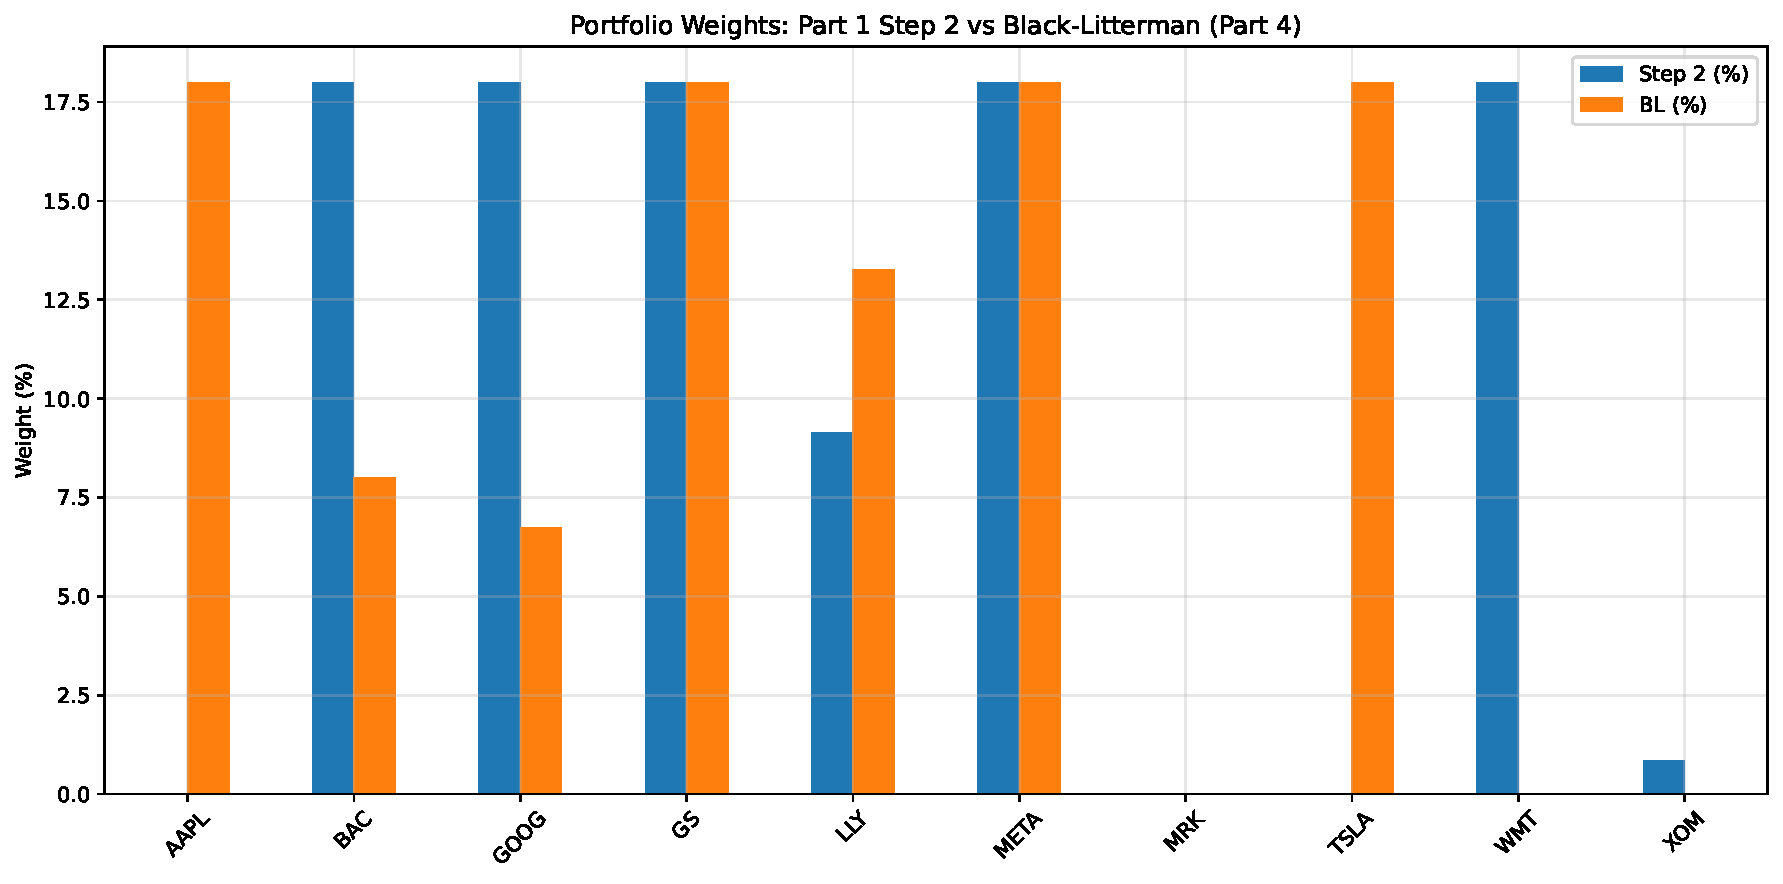
\includegraphics[width=0.95\textwidth]{bl_weights_comparison.pdf}
\caption{Portfolio weights: Part 1 Step 2 versus Black-Litterman model (Part 4)}
\label{fig:bl_comparison}
\end{figure}

The views increased allocations to TSLA and LLY while reducing exposure to WMT and BAC, demonstrating how investor opinions can meaningfully alter the optimal portfolio even under tight concentration constraints.

% ==================== END OF PART 4 ====================
\section{Conclusion and Practical Takeaways}
All in all, the number crunching shows that when you slap on the client’s 18\% cap and mix in your own hunches through the Black-Litterman blender, the portfolio just feels sturdier. We end up with a mix that keeps the return engine humming, keeps the risk gremlins quiet, and still stays buddies with the style factors we like while never letting any single stock hog more than about 18\% of the pie. In short: rules plus views equals a smoother ride, and that’s the combo we’d hand to a real-world client without loosing too much sleep.

\bibliographystyle{plainnat}
\begin{thebibliography}{99}
\bibitem{markowitz1952} Markowitz, H. (1952) ``Portfolio Selection''. \textit{Journal of Finance}, 7(1), pp. 77--91.
\bibitem{blacklitterman1992} Black, F. and Litterman, R. (1992) ``Global Portfolio Optimization''. \textit{Financial Analysts Journal}, 48(5), pp. 28--43.
\bibitem{famafrench2015} Fama, E.F. and French, K.R. (2015) ``A Five-Factor Asset Pricing Model''. \textit{Journal of Financial Economics}, 116(1), pp. 1--22.
\bibitem{french2026} French, K.R. (2026) ``Data Library''. Available at: \url{https://mba.tuck.dartmouth.edu/pages/faculty/ken.french/data_library.html} (Accessed: 10 May 2026).
\bibitem{ruppert2011} Ruppert, D. (2011) \textit{Statistics and Data Analysis for Financial Engineering}. Springer.
\end{thebibliography}

\end{document}